\documentclass[a4paper,10pt]{article}
%\usepackage[latin1]{inputenc} % Paquetes de idioma (otro encoding)
\usepackage[utf8]{inputenc} % Paquetes de idioma
\usepackage[spanish]{babel} % Paquetes de idioma
\usepackage{graphicx} % Paquete para ingresar gráficos
\usepackage{grffile}
\usepackage{hyperref}
\usepackage{fancybox}
\usepackage{amsmath}
\usepackage{amsfonts}
\usepackage{listings}
\usepackage{pdfpages}
% Paquetes de macros de Circuitos
%\usepackage{pstricks}
\usepackage{tikz}

% Encabezado y Pié de página
% Paquete para encabezados y pie de página
\usepackage{fancyhdr} 
% Sin esta línea no se imprimiría el encabezado en todas las páginas
\pagestyle{fancy} 

% Borra el encabezado anterior (Por defecto escribe el título de la 
%  sección en la que se encuentra la hoja
\fancyhf{} 
\setlength{\headheight}{22.55pt}
\fancyhead[L]{
	{\textsf{Facultad de Ingenieríaa $-$ Universidad de Buenos Aires 
    \\ 75.61 Taller de Programación III}}
}
%\addtocounter{page}{5}
\fancyhead[R]{\thepage}

% Ajusta el tamaño de las líneas separadoras en el pié de página
\renewcommand{\footrulewidth}{0.4pt}
 % Ajusta el tamaño de las líneas separadoras en el encabezado
\renewcommand{\headrulewidth}{0.4pt} 

\fancyfoot[L]{
	{\textsf{TP N$^{\circ}$2 - Ejercicio de Colas (RabbitMQ)} \\
	{\textsf{Integrantes: Torres Feyuk}}
	}
}
		

% Carátula del Trabajo
\title{ \author{} % Lo pongo para que el warning no moleste :p
\setlength{\unitlength}{1cm} %  Especifica la unidad de trabajo
\thispagestyle{empty}

\begin{picture}(18,0)
\put(0,0){
\includegraphics[width=1.5cm, height=3cm]{Imagenes/Logo1.png}}

\put(10.5,0){
\includegraphics[width=3cm, height=3cm]{Imagenes/Logo2.png}}

\end{picture}
\\[1.5cm]
\begin{center}
	\textbf{{\Huge Facultad de Ingeniería \\ Universidad de Buenos Aires}}
    \\[2cm]
	{75.61 Taller de Programación III}\\[0.5cm]
	{TP N$^{\circ}$2 - Ejercicio de Colas (RabbitMQ)}\\[2.5cm]
\end{center}

\begin{flushleft}
	\textbf{Profesor: Andrés Veiga} \\
    \textbf{JTP: Pablo Roca} \\[1cm]
	\textbf{Integrantes:} \\[1cm]

	\begin{tabular}{|c|c|c|}
		\hline
		\textbf{\normalsize Padrón} & \textbf{\normalsize Nombre} 
                                    & \textbf{\normalsize Email} \\
		\hline
		\normalsize 89579 & \normalsize Torres Feyuk, Nicolás R. Ezequiel 
                          & \normalsize ezequiel.torresfeyuk@gmail.com \\
		\hline
	\end{tabular}
\end{flushleft}
\date{} % Hace que no se imprima la fecha en la cual se compilo el .tex
 }

\begin{document}
	\maketitle % Hace que el título anterior sea el principal del documento
	\newpage

    % Esta línea genera un indice a partir de las secciones y 
    % subsecciones creadas en el documento
	\tableofcontents 
	\newpage

	\section{Introducción}
		El objetivo del presente trabajo práctico consiste en diseñar e 
        implementar un sistema de recepción de pedidos masivos. Para 
        realizar esta tarea, se deben implementar procesos que
        modelen diferentes partes/tareas del sistema. Para comunicar los 
        procesos, se deben utilizar cola de mensajes distribuidas. \\
        \indent RabbitMQ es un middleware orientado a mensajes el cual 
        permite conectar diferentes procesos a través de colas de mensajes
        distribuídas. 

    \newpage
    \section{Arquitectura 4 + 1}

    \newpage
    \subsection{Casos de Uso}

    \newpage
    \subsection{Vista Lógica}

    \newpage
    \subsection{Vista de Procesos}

    \newpage
    \subsection{Vista de Despliegue}
        Para la vista de despliegue se decidió realizar un diagrama de 
        robustez para explicar la arquitectura del sistema. El mismo se 
        puede visualizar en la figura \ref{DiagRobustez}. Debido a que
        no se encontro una herramienta adecuada para graficar el mismo,
        se detalla a continuación los elementos utilizados junto con el
        significado de cada uno:

        \begin{figure}[!htb]                                             
            \centering                                                   
            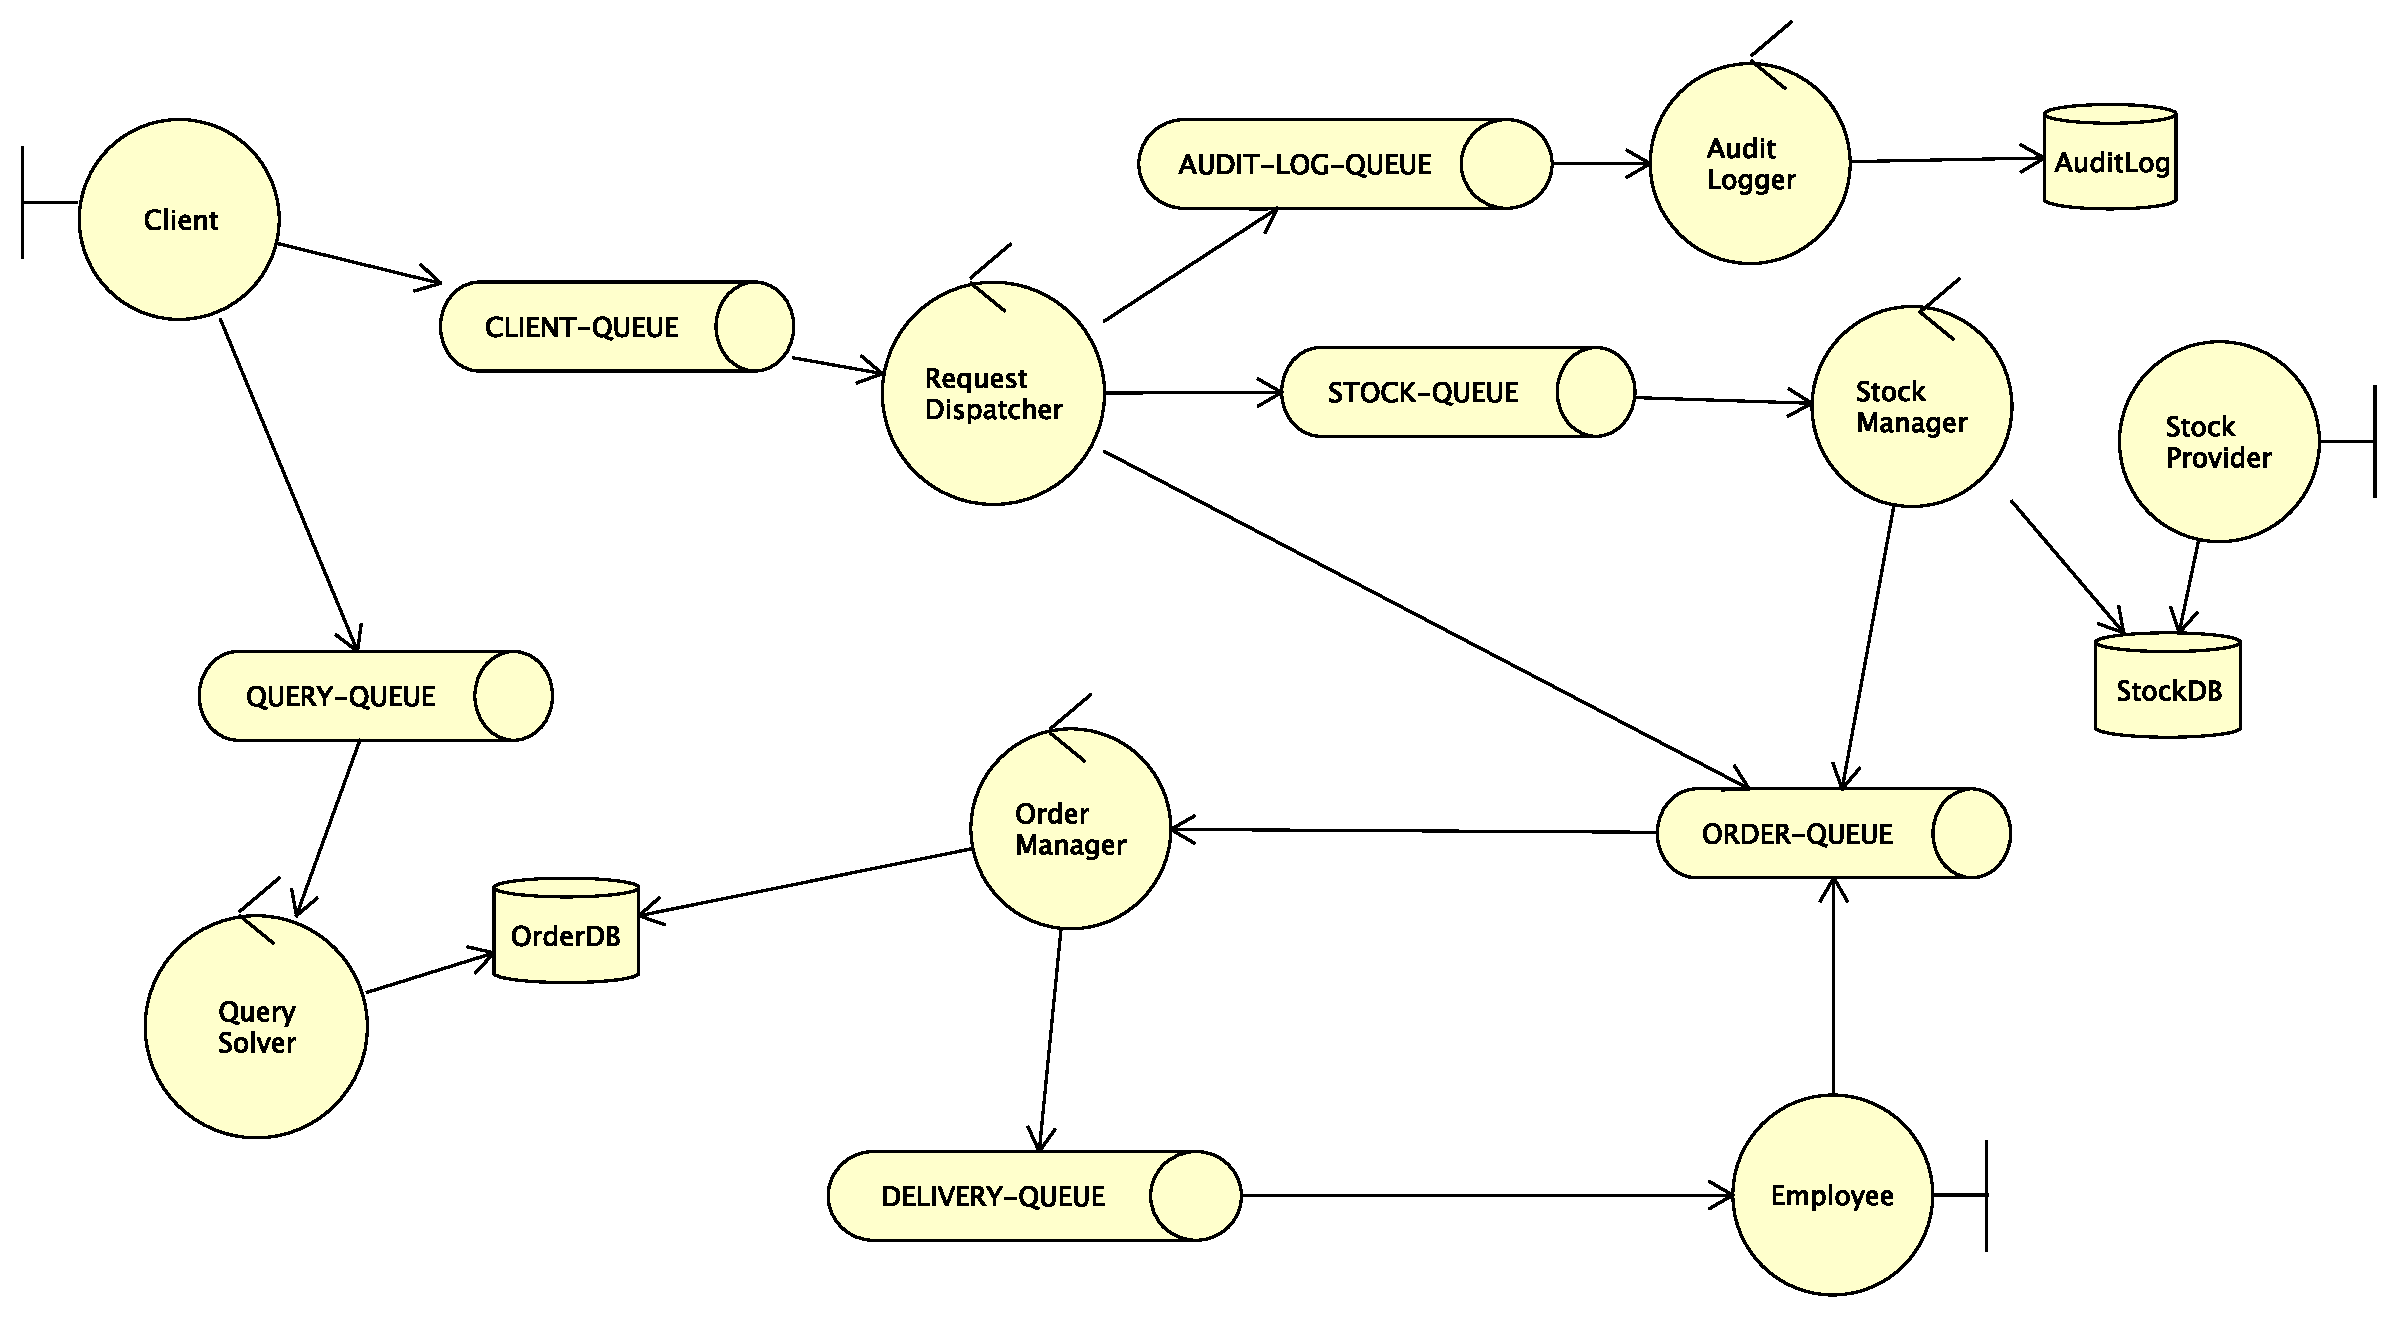
\includegraphics[width=20cm,angle=90,origin=c]{Imagenes/robustez.pdf}        
            \caption{Diagrama de Robustez} \label{DiagRobustez}
        \end{figure}

        \begin{itemize}
            \item \textbf{Círculos Rojos:} Procesos que envían estímulos al 
            sistema
            \item \textbf{Círculos Verdes:} Controladores. Puede haber N 
            de ellos          
            \item \textbf{Círculos Amarillos:} Controladores. Por cuestiones
            de modelo de negocio, solo puede haber uno de estos controladores
            de cada tipo al mismo tiempo
            \item \textbf{Colas:} RabbitMQ Queues. Las flechas entrantes 
            indican que un controlador ingresa mensajes en la cola. Flechas
            salientes indican que un controlador saca elementos de la cola.
            \item \textbf{Discos:} Archivos físicos los cuales, en el presente
            trabajo, simulan el funcionamiento de bases de datos relacionales.
        \end{itemize}

   
    %\newpage 
    %\section{Código}
    %    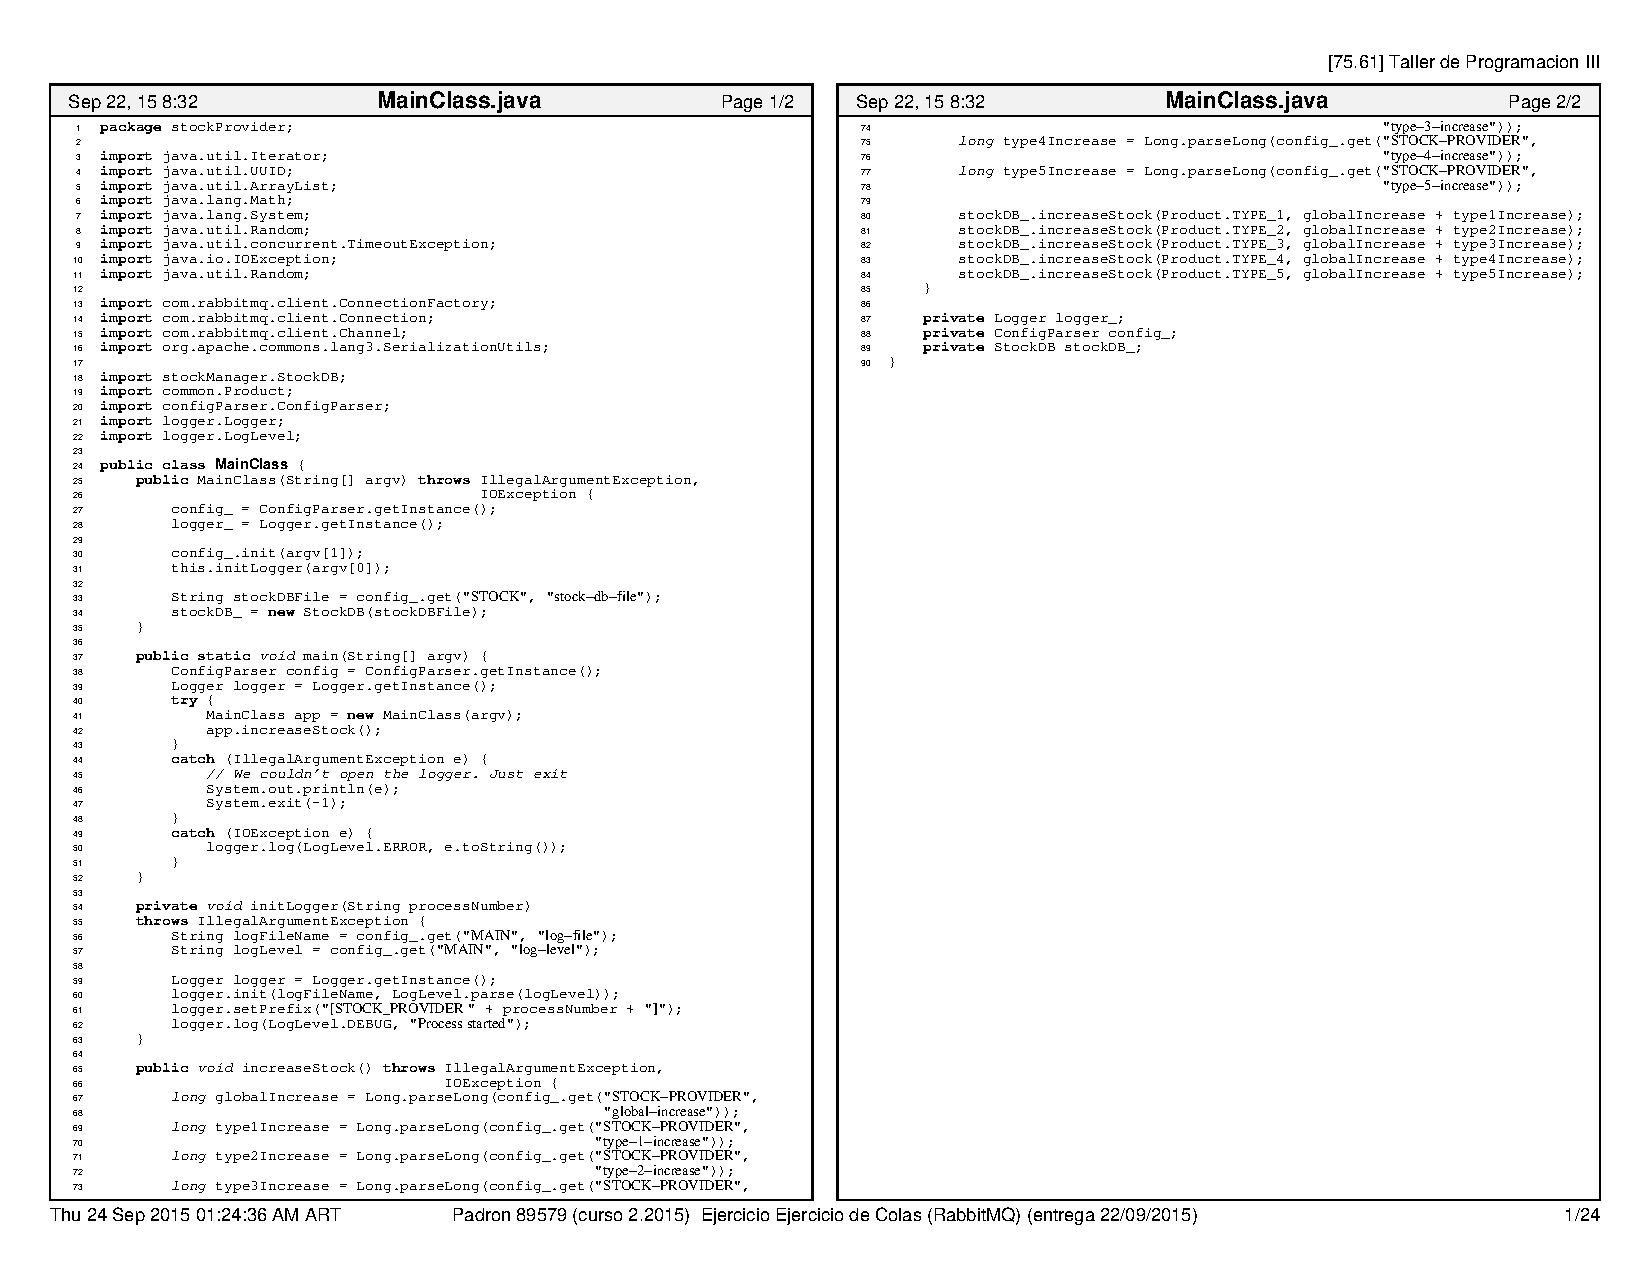
\includepdf[pages=-,scale=.8,pagecommand={},landscape=true]{codigo.pdf}
\end{document}

